\documentclass[11pt]{beamer}

\usetheme{Madrid}
\usecolortheme{dolphin}
\definecolor{myyellow}{HTML}{FFCC5F}
\setbeamercolor{background canvas}{bg=myyellow}

% * conseguir manusear uma variedade de símbolos usados nos diferentes grupos de línguas
\usepackage[latin1,utf8]{inputenc}

\usepackage[portuguese]{babel}

% * colorir textos
\usepackage{graphicx}

% * multiplas colunas
\usepackage{multicol}

\usepackage{xcolor,colortbl} % * Cores nas células
\usepackage{booktabs, multirow} % * Para bordas das tabelas
\usepackage{soul}% * Para o sublinhado
\usepackage{changepage,threeparttable} % * Tabelas largas.

\title{Finanças pessoais}
\author{Arthur Aguiar - 64726}
\date{24 de Novembro de 2024}

\begin{document}
	\maketitle

	% * Tabela Resumo e o gráfico Rendimentos vs Gastos
	\begin{frame}{Rendimentos vs Gastos}
		\begin{table}[!h]\centering
			\tiny
			\begin{tabular}{lrrrrrrrr}\toprule
				RESUMO &Setembro &Outubro &Novembro &Dezembro &Janeiro &Fevereiro &TOTAL \\\midrule
				\cellcolor[HTML]{4285f4}Rendimentos &729.80€ &729.80€ &729.80€ &729.80€ &729.80€ &729.80€ &\cellcolor[HTML]{4285f4}4,378.80€ \\
				\cellcolor[HTML]{4285f4}Gastos &687.00€ &550.00€ &587.00€ &600.00€ &520.00€ &510.00€ &\cellcolor[HTML]{4285f4}3,454.00€ \\
				\cellcolor[HTML]{4285f4}Saldo do Mês &42.80€ &179.80€ &142.80€ &129.80€ &209.80€ &219.80€ &\cellcolor[HTML]{4285f4}924.80€ \\
				\cellcolor[HTML]{4285f4}Saldo Acumulado &42.80€ &222.60€ &365.40€ &495.20€ &705.00€ &924.80€ &\cellcolor[HTML]{4285f4}924.80€ \\
				\bottomrule
			\end{tabular}
			\caption{Resumo das finanças pessoais}\label{tab:resumo }
		\end{table}

		\begin{figure}
			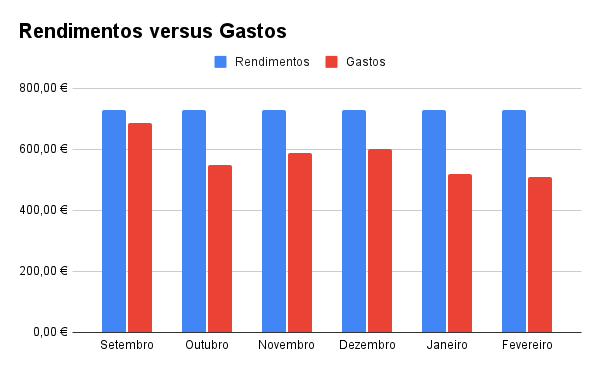
\includegraphics[width=5cm]{./rendimentos_gastos_grafico_barra.png}
			\caption{Rendimentos vs Gastos}\label{fig:barra}
		\end{figure}
	\end{frame}

	% *Tabela as contas e o gráfico correspondente
	\begin{frame}{Despesas/contas}

		\begin{multicols}{2}			
			\begin{table}[!h]\centering
				\scriptsize
				\begin{tabular}{lrr}\toprule
					As Contas &TOTAL \\\midrule
					Rendimentos & 4,378.80€ \\
					Habitação & 2,280.00€ \\
					Saúde & 150.00€ \\
					Transportes & 80.00€ \\
					Despesas Pessoais & 258.00€ \\
					Lazer & 94.00€ \\
					Ensino & 562.00€ \\
					Extras & 30.00€ \\
					\bottomrule
				\end{tabular}
				\caption{Contas}\label{tab:contas}
			\end{table}
	
			\begin{figure}
				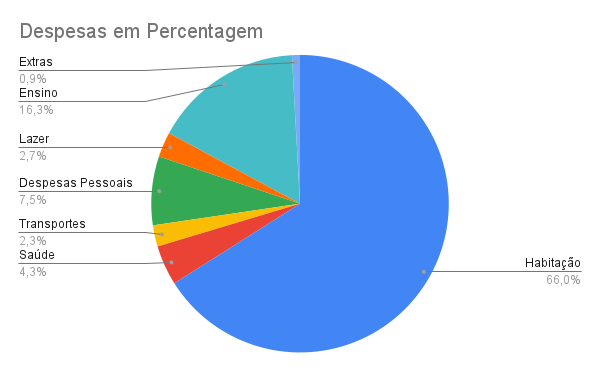
\includegraphics[width=5cm]{./despesas_percentagem.png}
				\caption{Despesas percentagem}\label{fig:circular}
			\end{figure}
		\end{multicols}
	\end{frame}

	% * Topicos e esquemas para explicar o racionio de como que eu fiz para colocar
	% * a tabela planeamento
	\begin{frame}[ allowframebreaks ]{Planeamento explicação}

		\begin{table}[!htp]\centering
			\tiny
			\begin{tabular}{lrrrrrrrr}\toprule
				PLANEAMENTO &Setembro &Outubro &Novembro &Dezembro &Janeiro &Fevereiro &TOTAL \\\midrule
				Salário &820.00€ &820.00€ &820.00€ &820.00€ &820.00€ &820.00€ &\cellcolor[HTML]{4285f4}4,920.00€ \\
				\cellcolor[HTML]{4285f4}RENDIMENTOS &\cellcolor[HTML]{4285f4}729.80€ &\cellcolor[HTML]{4285f4}729.80€ &\cellcolor[HTML]{4285f4}729.80€ &\cellcolor[HTML]{4285f4}729.80€ &\cellcolor[HTML]{4285f4}729.80€ &\cellcolor[HTML]{4285f4}729.80€ &\cellcolor[HTML]{4285f4}4,378.80€ \\
				& & & & & & & \\
				\cellcolor[HTML]{4285f4}HABITAÇÃO &\cellcolor[HTML]{4285f4}380.00€ &\cellcolor[HTML]{4285f4}380.00€ &\cellcolor[HTML]{4285f4}380.00€ &\cellcolor[HTML]{4285f4}380.00€ &\cellcolor[HTML]{4285f4}380.00€ &\cellcolor[HTML]{4285f4}380.00€ &\cellcolor[HTML]{4285f4}2,280.00€ \\
				Aluguer &250.00€ &250.00€ &250.00€ &250.00€ &250.00€ &250.00€ &\cellcolor[HTML]{4285f4}1,500.00€ \\
				Supermercado &100.00€ &100.00€ &100.00€ &100.00€ &100.00€ &100.00€ &\cellcolor[HTML]{4285f4}600.00€ \\
				Alimentação &30.00€ &30.00€ &30.00€ &30.00€ &30.00€ &30.00€ &\cellcolor[HTML]{4285f4}180.00€ \\
				& & & & & & & \\
				\cellcolor[HTML]{4285f4}SAÚDE &\cellcolor[HTML]{4285f4}60.00€ &\cellcolor[HTML]{4285f4}20.00€ &\cellcolor[HTML]{4285f4}20.00€ &\cellcolor[HTML]{4285f4}20.00€ &\cellcolor[HTML]{4285f4}20.00€ &\cellcolor[HTML]{4285f4}10.00€ &\cellcolor[HTML]{4285f4}150.00€ \\
				Médicos &50.00€ & & & & & &\cellcolor[HTML]{4285f4}50.00€ \\
				Medicamentos &10.00€ &20.00€ &20.00€ &20.00€ &20.00€ &10.00€ &\cellcolor[HTML]{4285f4}100.00€ \\
				& & & & & & & \\
				\cellcolor[HTML]{4285f4}TRANSPORTES &\cellcolor[HTML]{4285f4}10.00€ &\cellcolor[HTML]{4285f4}10.00€ &\cellcolor[HTML]{4285f4}30.00€ &\cellcolor[HTML]{4285f4}10.00€ &\cellcolor[HTML]{4285f4}10.00€ &\cellcolor[HTML]{4285f4}10.00€ &\cellcolor[HTML]{4285f4}80.00€ \\
				Passe & & & & & & &\cellcolor[HTML]{4285f4}0.00€ \\
				Camioneta &10.00€ &10.00€ &10.00€ &10.00€ &10.00€ &10.00€ &\cellcolor[HTML]{4285f4}60.00€ \\
				Comboio & & &20.00€ & & & &\cellcolor[HTML]{4285f4}20.00€ \\
				& & & & & & & \\
				\cellcolor[HTML]{4285f4}DESPESAS PESSOAIS &\cellcolor[HTML]{4285f4}28.00€ &\cellcolor[HTML]{4285f4}58.00€ &\cellcolor[HTML]{4285f4}58.00€ &\cellcolor[HTML]{4285f4}58.00€ &\cellcolor[HTML]{4285f4}28.00€ &\cellcolor[HTML]{4285f4}28.00€ &\cellcolor[HTML]{4285f4}258.00€ \\
				Higiene Pessoal &13.00€ &13.00€ &13.00€ &13.00€ &13.00€ &13.00€ &\cellcolor[HTML]{4285f4}78.00€ \\
				Vestuário & &30.00€ &30.00€ &30.00€ & & &\cellcolor[HTML]{4285f4}90.00€ \\
				Telemóvel, Internet &15.00€ &15.00€ &15.00€ &15.00€ &15.00€ &15.00€ &\cellcolor[HTML]{4285f4}90.00€ \\
				& & & & & & & \\
				\bottomrule
			\end{tabular}
			\caption{Planeamento das finanças pessoais, parte I.}\label{tab:planeamento1 }
		\end{table}


		\begin{table}[!htp]\centering
			\tiny
			\begin{tabular}{lrrrrrrrr}\toprule
				\cellcolor[HTML]{4285f4}LAZER &\cellcolor[HTML]{4285f4}22.00€ &\cellcolor[HTML]{4285f4}7.00€ &\cellcolor[HTML]{4285f4}24.00€ &\cellcolor[HTML]{4285f4}27.00€ &\cellcolor[HTML]{4285f4}7.00€ &\cellcolor[HTML]{4285f4}7.00€ &\cellcolor[HTML]{4285f4}94.00€ \\
				Restaurantes &15.00€ & &10.00€ &20.00€ & & &\cellcolor[HTML]{4285f4}45.00€ \\
				Bares & & & & & & &\cellcolor[HTML]{4285f4}0.00€ \\
				Cinema &7.00€ &7.00€ &14.00€ &7.00€ &7.00€ &7.00€ &\cellcolor[HTML]{4285f4}49.00€ \\
				& & & & & & & \\
				\cellcolor[HTML]{4285f4}ENSINO &\cellcolor[HTML]{4285f4}187.00€ &\cellcolor[HTML]{4285f4}75.00€ &\cellcolor[HTML]{4285f4}75.00€ &\cellcolor[HTML]{4285f4}75.00€ &\cellcolor[HTML]{4285f4}75.00€ &\cellcolor[HTML]{4285f4}75.00€ &\cellcolor[HTML]{4285f4}562.00€ \\
				Propinas e Taxas &157.00€ &60.00€ &60.00€ &60.00€ &60.00€ &60.00€ &\cellcolor[HTML]{4285f4}457.00€ \\
				Material Escolar &30.00€ &15.00€ &15.00€ &15.00€ &15.00€ &15.00€ &\cellcolor[HTML]{4285f4}105.00€ \\
				Livros &40.00€ &8.00€ &10.00€ &15.00€ & & &\cellcolor[HTML]{4285f4}73.00€ \\
				& & & & & & & \\
				\cellcolor[HTML]{4285f4}EXTRAS &\cellcolor[HTML]{4285f4}- &\cellcolor[HTML]{4285f4}- &\cellcolor[HTML]{4285f4}- &\cellcolor[HTML]{4285f4}30.00€ &\cellcolor[HTML]{4285f4}- &\cellcolor[HTML]{4285f4}- &\cellcolor[HTML]{4285f4}30.00€ \\
				& & & &30.00€ & & &\cellcolor[HTML]{4285f4}30.00€ \\
			\end{tabular}
			\caption{Planeamento das finanças pessoais, parte II.}\label{tab:planeamento2 }
		\end{table}

		\allowbreak{}
		
		\large{
			\textbf{Como fazer a tabela planeamento encaixar dentro do frame}
		}
		\begin{enumerate}
			\normalsize
			\item Copíe e cole a tabela dentro do frame;
			\item Alterei o tamanho da letra de \textbf{scriptsize} para \textbf{tiny};
			\item Divide a tabela em duas partes e crie novas tabelas respectivamente.
		\end{enumerate}
	\end{frame}

	\begin{frame}{Imagem relacionada ao tema}
		\begin{figure}
			
\includegraphics[width=5cm]{./foca_financeiro.jpg}
			\caption{\url{https://br.pinterest.com/pin/503769908314307626/}}
		\end{figure}
	\end{frame}
\end{document}